\documentclass[11pt,a4paper]{article}

\usepackage[utf8]{inputenc} 
\usepackage[T1]{fontenc} 
\usepackage[spanish]{babel}
\decimalpoint
\setlength{\parskip}{0.5\baselineskip} 
\usepackage{fullpage}
\usepackage[procnames]{listings}
\usepackage{fancyhdr}
\usepackage{lastpage}
\usepackage{xcolor}
\usepackage{graphicx}
\usepackage{subcaption}
\usepackage[fleqn]{amsmath}
\parindent 0in 
\setlength{\mathindent}{0pt}


%% DEFINICIONES
\newcommand{\TODO}[1]{{\huge \color{red} \textbf{TODO: }#1 }}
\newcommand{\todo}[1]{{\large \color{red} \textbf{TODO: }#1 }}



\begin{document} 
\pagestyle{fancy}
\fancyhf{}
\lhead{P2: k-means (aparatado B)}
\rhead{Luis Mª Costero Valero, Jesús J. Doménech Arellano}
\rfoot{\thepage\ / \pageref{LastPage}}
\renewcommand{\headrulewidth}{0.4pt}
\renewcommand{\footrulewidth}{0.4pt}
\section*{}

\textbf{Implementar las 3 medidas de cohesión (radio, diámetro y distancia al
cuadrado promedio con respecto el centroide) para evaluar la calidad del
clustering para valores de k entre 2 y 20. Visualizar la variación de la
cohesión como un gráfico de líneas para cada una de las medidas y razonar
cuál podría ser un buen valor de k.}


En la figuras~\ref{fig:radio},~\ref{fig:diametro}~y~\ref{fig:promedio} se
muestra la evolución de las medidas de radio, diámetro y distancia al
cuadrado promedio según se incrementa el número de clusters (K). La distancia
al cuadrado promedio se ha calculado teniendo en cuenta todas las
instancias con sus respectivos centroides, mientras que el radio y el
diámetro se ha realizado calculando la media aritmética entre el radio (o
diámtero) de todos los clusters. Así mismo, en estas dos últimas gráficas
se muestra la distancia máxima y mínima entre todos los clusters. 




%% A lo mejor esto sería interesante cambiarlo y ponerlo de alguna forma
%% chula, estilo 2/1, o 1/2 o 3/0 o algo así
\begin{figure}[h]
\begin{subfigure}{0.45\textwidth}
  \centering
 %%----primera subfigura---- 
    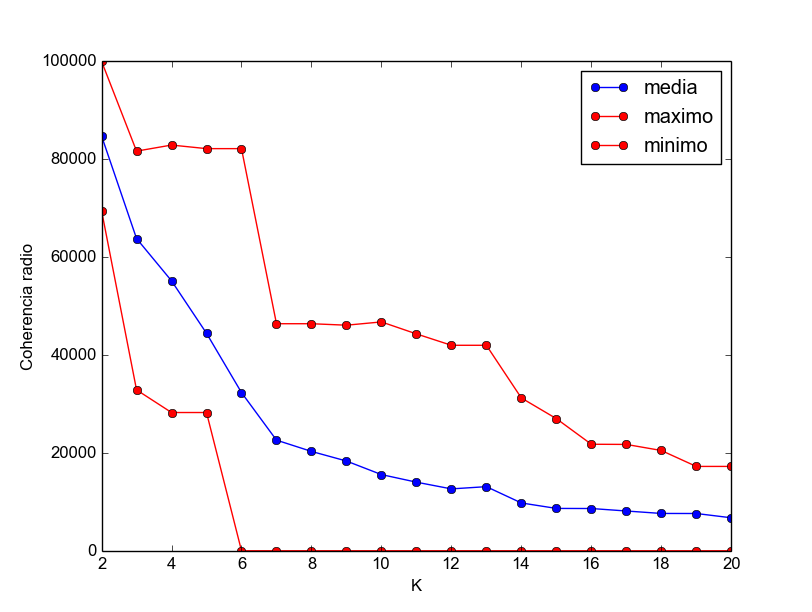
\includegraphics[width=0.9\textwidth]{img/radio_maxMin.png}
    \caption{Evolución del radio según aumenta el número de clusters}
    \label{fig:radio} 
\end{subfigure}
\hspace{0.1\textwidth}
\begin{subfigure}{0.45\textwidth}
  %% ----segunda subfigura----
    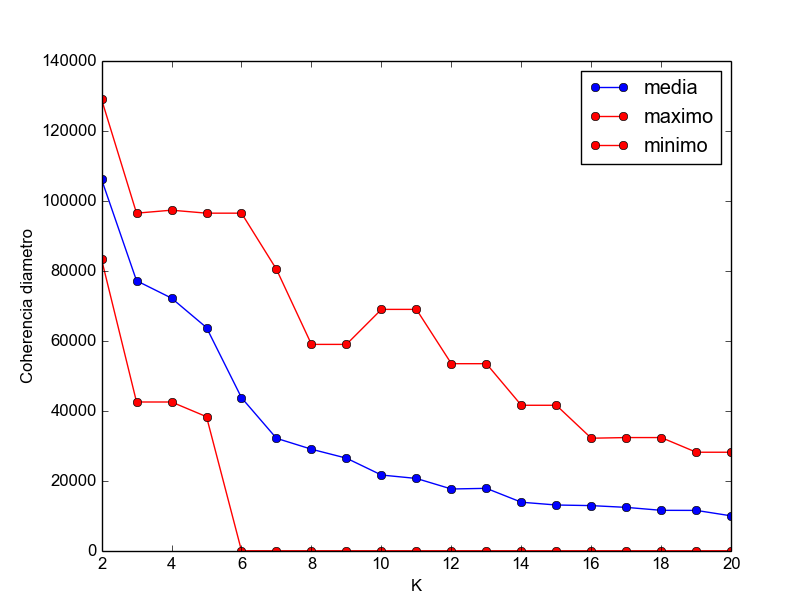
\includegraphics[width=0.9\textwidth]{img/diametro_maxMin.png}
    \caption{Evolución del diámetro según aumenta el número clusters}
    \label{fig:diametro}
\end{subfigure}
\begin{subfigure}{\textwidth}
  %% ----tercera subfigura----
  \centering
    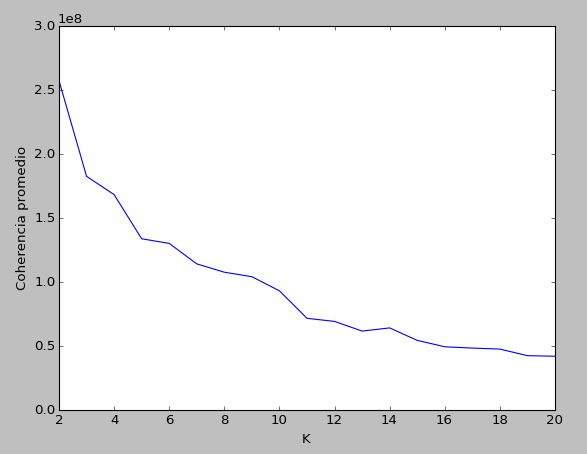
\includegraphics[width=0.45\textwidth]{img/figure_P.png}
    \caption{Evolución de la distancia al cuadrado promedio según aumenta el número de clusters}
    \label{fig:promedio}
  \end{subfigure}

\end{figure}



%%\hrule
%%\hrule


Se puede observar como a partir de cierto número de clusters, la distancia
mínima tiende (o es) 0, y la máxima también va decreciendo, ya que existen
clusters donde las instancias coinciden con el centroide o se
encuentran muy próximas a él. \\

Trás realizar el experimento proponemos escoger $K = 8$, dado que las
distancias máximas han bajado lo suficiente en las tres medidas, y
empiezan a haber clusters muy  pequeños. Además tenemos en cuenta que
a mayor número de clusters objetivo el tiempo de ejecución es mayor y
la mejora no es significativa. Aunque, por supuesto, la elección de
$K$ depende del problema a resolver.
\end{document}
